%!TEX root = ../dissertation.tex
%\begin{savequote}[75mm]
%Nulla facilisi. In vel sem. Morbi id urna in diam dignissim feugiat. Proin molestie tortor eu velit. Aliquam erat volutpat. Nullam ultrices, diam tempus vulputate egestas, eros pede varius leo.
%\qauthor{Quoteauthor Lastname}
%\end{savequote}

\chapter{Evaluation and Results}
This chapter will first explain the configuration and results of the experiments used to determine the vocabulary size (Section \ref{sec:4-vocab_size}) and sentence length (Section \ref{sec:4-sentence_length}). Following this are details of experiments for the Baseline model (Section \ref{sec:4-baseline}), Trivial Transfer Learning model (Section \ref{sec:4-trivial}), and Hierarchical Transfer Learning model (Section \ref{sec:4-hierarchical}).
\newpage

\section{Experiments}

The Scottish Gaelic dataset consists of 145,000 sentences from the the original and back-translated data, as described in Table \ref{tab:low_resource-data}. The French dataset consists of 170,000 sentences from the data described in Table \ref{tab:available-data}. Finally the Irish Gaelic dataset consists of 165,000 sentences from the back-translated monolingual English data extracted from the Italian and Spanish data described in Table \ref{tab:available-data}.
All of the sentences fit within the maximum sentence length of 20 words and as mentioned in the methodology.
For the parent and intermediary languages, the test split been set to 0 and the validation split has been set to 0.1. This means that a significantly higher percentage of the available sentences are used for training. In line with the existing transfer learning research identified in the literature review, parent models were trained for 5 epochs before switching the dataset to child languages.

% ======================================================

\subsection{Vocabulary Size}
\label{sec:4-vocab_size}

During data pre-processing, the source and target language vocabulary size have been limited, with prioritisation given to the most frequently occurring words. To determine the most suitable vocabulary size for the full Scottish Gaelic dataset with 145,000 sentences, tests at sizes 4000, 5000, and 7000 were completed. Due to the total vocabulary size with a minimum word occurrence of 2 totalling approximately 7000, the maximum possible size for this dataset is 7000. 
The vocabulary size of subsequent experiments will be determined by selecting the vocabulary size that returns highest \acrshort{BLEU} score. The validation loss during training and \acrshort{BLEU} score of each size is shown in Figure \ref{fig:vocab_loss_bleu}.

\begin{figure}[ht!]
\centering
\makebox[\textwidth][c]{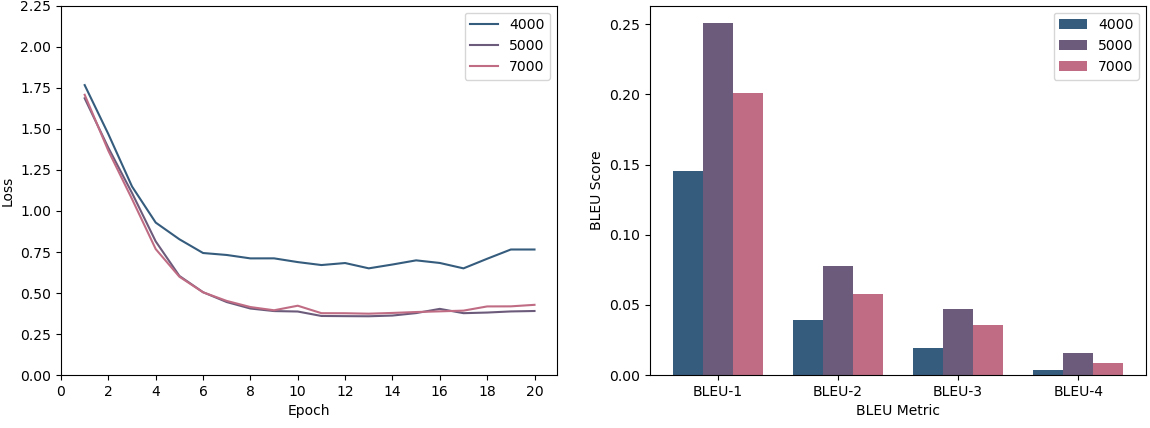
\includegraphics[width=1.15\textwidth]{media/experiments/bleu/vocab_loss_bleu.jpg}}
\captionsetup{justification=centering}
\caption[Vocabulary size validation loss and BLEU score]{Vocabulary size. Left side: Validation loss. Right side: BLEU score}
\label{fig:vocab_loss_bleu}
\end{figure}

% ======================================================

\subsection{Sentence Length}
\label{sec:4-sentence_length}

As mentioned previously, padding is added to any sentence with less words than the longest sentence. To determine the most suitable sentence length for the Scottish Gaelic dataset, tests at sizes 15 and 20 were completed. These values were selected based on the analysis of the dataset in Figure \ref{fig:sentence_length-gaelic}, where the majority of sentences fall within a 15 word limit, with an additional 6,000 sentences between 16 and 20. This experiment will reveal whether a reduction in the overall variable length sequence padding improves the translation quality.
139,000 sentences from the Scottish Gaelic dataset were used for both sizes, using the vocabulary size of 5000 as determined by the result of the previous experiment. Subsequent experiments will use the sentence length that the yields highest \acrshort{BLEU} score. The validation loss and \acrshort{BLEU} score of each sentence length is shown in Figure \ref{fig:length_loss_bleu}.

\begin{figure}[ht!]
\centering
\makebox[\textwidth][c]{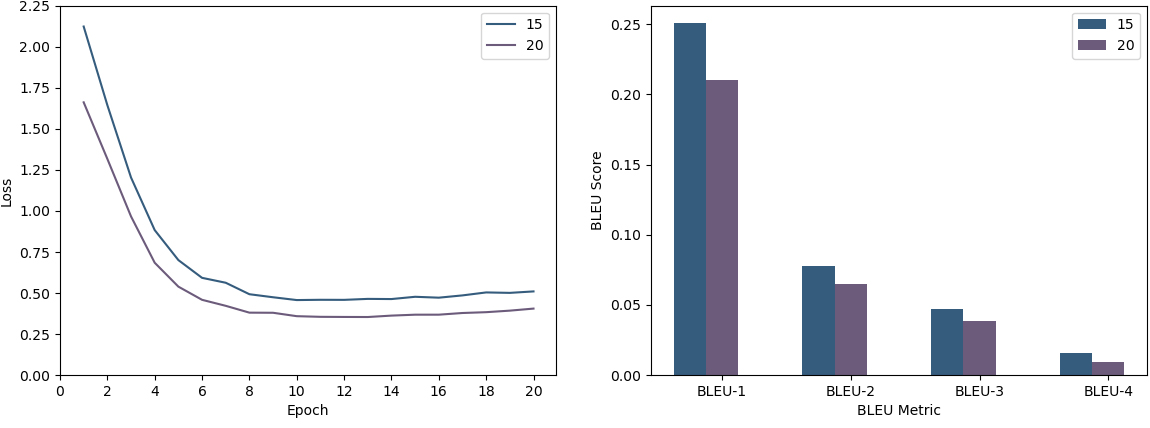
\includegraphics[width=1.15\textwidth]{media/experiments/bleu/length_loss_bleu.jpg}}
\captionsetup{justification=centering}
\caption[Sentence length validation loss and BLEU score]{Sentence length. Left side: Validation loss. Right side: BLEU score}
\label{fig:length_loss_bleu}
\end{figure}

% ======================================================

\subsection{Baseline}
\label{sec:4-baseline}

The baseline translation model described in Section \ref{sec:3-model} has been trained for 20 epochs with a vocabulary size of 5000 using 139,000 sentences from Scottish Gaelic dataset with a maximum sentence length of 15. The training and validation loss can be seen in Figure \ref{fig:loss_baseline}.

\begin{figure}[ht!]
\centering
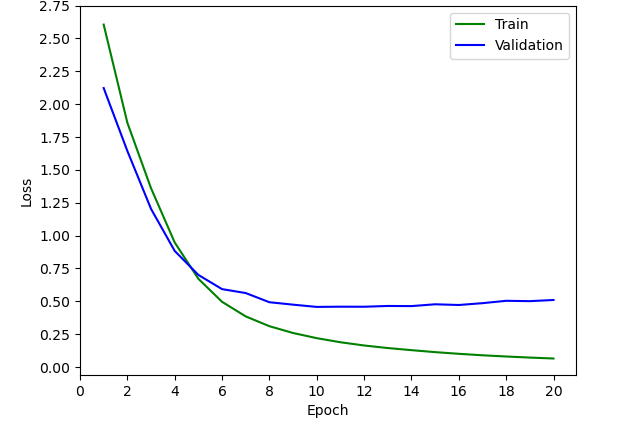
\includegraphics[width=0.65\textwidth]{media/experiments/loss/5k/loss_baseline.png}
\captionsetup{justification=centering}
\caption[Baseline Model Training \& Validation Loss]{Baseline Model Training \& Validation Loss}
\label{fig:loss_baseline}
\end{figure}

% ======================================================

\subsection{Trivial Transfer Learning}
\label{sec:4-trivial}

The trivial transfer learning method that is described in Section \ref{sec:2-transfer_learning} has been implemented using a vocabulary size of 5000 and maximum sentence length of 15 using 170,000 sentences from the French dataset as the parent language and 139,000 sentences from the Gaelic dataset as the child language. The parent language was trained for 5 epochs, initialising the child language that was trained for a further 15 epochs. The training and validation loss is shown in Figure \ref{fig:loss_trivial}, where a spike is present after 5 epochs as a result of switching from French to Gaelic.

\begin{figure}[ht!]
\centering
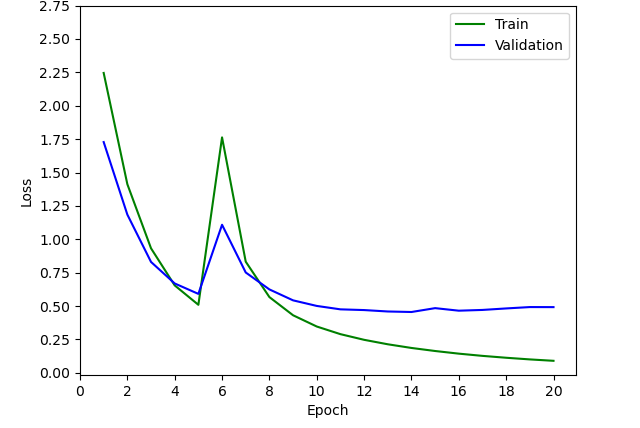
\includegraphics[width=0.65\textwidth]{media/experiments/loss/5k/loss_trivial.png}
\captionsetup{justification=centering}
\caption[Baseline Model Training \& Validation Loss]{Trivial Transfer Learning Model Training \& Validation Loss}
\label{fig:loss_trivial}
\end{figure}

% ======================================================


\subsection{Hierarchical Transfer Learning}
\label{sec:4-hierarchical}

The hierarchical transfer learning approach described in Section \ref{sec:2-transfer_learning} has been implemented using French as the parent language, Irish Gaelic as the intermediary language and Scottish Gaelic as the child language. Both the French dataset and Irish Gaelic dataset include 170,000 sentences. The French parent was trained for 5 epochs, then the data was switched to Irish Gaelic and trained for another 5 epochs before finally training on Scottish Gaelic data for 10 epochs. Spikes in the training and validation scores are observed on epochs where the dataset has been switched, as shown in Figure \ref{fig:loss_hierarchical}.


\begin{figure}[ht!]
\centering
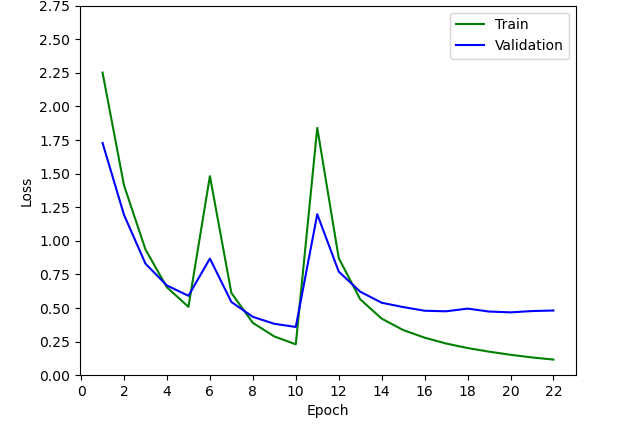
\includegraphics[width=0.65\textwidth]{media/experiments/loss/5k/loss_hierarchical.png}
\captionsetup{justification=centering}
\caption[Baseline Model Training \& Validation Loss]{Hierarchical Transfer Learning Model Training \& Validation Loss}
\label{fig:loss_hierarchical}
\end{figure}

% ======================================================

%\newpage
%\section{Results}
%\label{sec:4-results}

\begin{figure}[!ht]
\centering
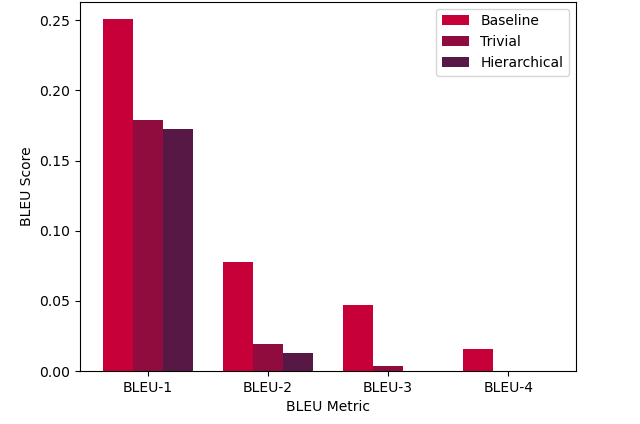
\includegraphics[width=0.70\textwidth]{media/experiments/bleu/5k_bleu.png}
\captionsetup{justification=centering}
\caption[Model BLEU scores]{Model BLEU scores}
\label{fig:bleu_results}
\end{figure}

\begin{table}[!ht]
\centering
\setlength\doublerulesep{2pt}
\renewcommand{\arraystretch}{1.1}
\begin{longtable}{|l|l|l|l|l|l|}
\hline
\textbf{Model} & \textbf{BLEU-1} & \textbf{BLEU-2} & \textbf{BLEU-3} & \textbf{BLEU-4} & \textbf{NIST}\\ \hline
\endhead
%
\hline
\endfoot
%
\endlastfoot
%
Baseline       & 0.2507 & 0.0775 & 0.0469 & 0.0157 & 1.1978 \\
Trivial        & 0.1789 & 0.0196 & 0.0033 & 0.0004 & 0.7698 \\
Hierarchical   & 0.1723 & 0.0133 & 0.0000 & 0.0000 & 0.7814 \\ \hline
\captionsetup{justification=centering}
\caption{Translation evaluation scores}
\label{tab:bleu_table}\\
\end{longtable}
\end{table}


\begin{table}[!ht]
\centering
\setlength\doublerulesep{2pt}
\renewcommand{\arraystretch}{1.1}
%\begin{tabular}{|l|p{8cm}|}
\begin{tabular}{|l|l|}
\hline
\multicolumn{2}{|l|}{\textbf{Gaelic \textrightarrow \space English Translation}} \\ \hline
Source          & an t eun a tha marbh \\ \hline
Reference       & the bird is dead \\ \hline
Baseline        & the unk is the unk \\ \hline
Trivial         & are nothing t a would is \\ \hline
Hierarchical    & he don a would this to is \\ \hhline{==}
Source          & tha e na chadal   \\ \hline
Reference       & he s asleep   \\ \hline
Baseline        & the unk is the unk   \\ \hline
Trivial         & he in a him would lot are nothing \\ \hline
Hierarchical    & he in a   \\\hline
\end{tabular}
\captionsetup{justification=centering}
\caption{Translation sentence analysis}
\label{tab:sentence_analysis}
\end{table}

%Source          & feumaidh tu deise ur a cheannach airson an aodach obair agad agallamh   \\ \hline
%Reference       & you need to buy a new suit to wear to your job interview   \\ \hline
%Baseline        & i don t want to do you want to do you   \\ \hline
%Trivial         & s is a need this to two you to hear   \\ \hline
%Hierarchical    & s is a need this to two you to hear   \\ \hhline{==}
%Source          & an t uisge a bha blath   \\ \hline
%Reference       & the water was warm   \\ \hline
%Baseline        & i m not to do you do you   \\ \hline
%Trivial         & to water is a   \\ \hline
%Hierarchical    & to water is a   \\ \hline
